\documentclass{article}
\usepackage[utf8]{vietnam}
\usepackage[12pt]{extsizes}
\usepackage{amsmath,amsfonts,amsthm}
\usepackage{mathrsfs}
\usepackage{enumitem}
\usepackage{geometry}
\usepackage{mathtools}
\usepackage{booktabs}
\usepackage{pgfplots}
 \geometry{
 a4paper,
 total={170mm,257mm},
 left=20mm,
 top=20mm,
 }
 \usepackage{graphicx}
 \usepackage{titling}
 \title{Bài tập cộng điểm giữa kì
}
\author{Vũ Hàn Tín 23020874}
\date{Ngày 18/4/2025}
 \usepackage{fancyhdr}
\fancypagestyle{plain}{%  the preset of fancyhdr 
    \fancyhf{} % clear all header and footer fields
    \fancyfoot[L]{\thedate}
    \fancyhead[L]{ELT 3144: Xử lý tín hiệu số}
    \fancyhead[R]{\theauthor}
}
\makeatletter\def\@maketitle{%
\newpage
\null
\vskip 1em%
\begin{center}%
\let \footnote \thanks
  {\LARGE \@title \par}%
  \vskip 1em%
  %{\large \@date}%
\end{center}%
\par
\vskip 1em}
\makeatother
\begin{document}
\maketitle
\section{Chứng minh công thức của $\sigma$ và $\Omega$ từ phép biến đổi song tuyến tính.}
Ta có:
\begin{equation*}
    \begin{split}
        p&=C\frac{1-z^{-1}}{1+z^{-1}}=C\frac{z-1}{z+1}=C\frac{re^{j\omega}-1}{re^{j\omega}+1}=C\frac{(re^{j\omega}-1)(re^{-j\omega}+1)}{(re^{j\omega}+1)(re^{-j\omega}+1)}\\&=C\frac{r^{2}+2rj\sin{\omega}-1}{r^{2}+2r\cos{\omega}+1}=C\frac{r^2-1}{r^2+2r\cos{\omega}+1}+jC\frac{2r\sin{\omega}}{r^2+2r\cos{\omega}+1}
    \end{split}
\end{equation*}
Vậy ta suy ra:
\begin{equation*}
    \begin{split}
        \Re(p)&=\sigma=C\frac{r^2-1}{r^2+2r\cos{\omega}+1}\\ \Im(p)&=\Omega=C\frac{2r\sin{\omega}}{r^2+2r\cos{\omega}+1}
    \end{split}
\end{equation*}
\section{Tìm $C$ để $\Omega$ và $\omega$ liên hệ tuyến tính với nhau.}
Bản chất của phép biến đổi song tuyến tính (Bilinear Transformation) là phép biến đổi giữa miền Laplace và miền Z. 
Ta có thể minh họa hình học phép biến đổi này bằng cách lấy một điểm $s=\sigma+j\Omega$ tùy ý trên miền Laplace và chuyển nó sang miền Z tương ứng.
\begin{figure}[h]
    \begin{center}
    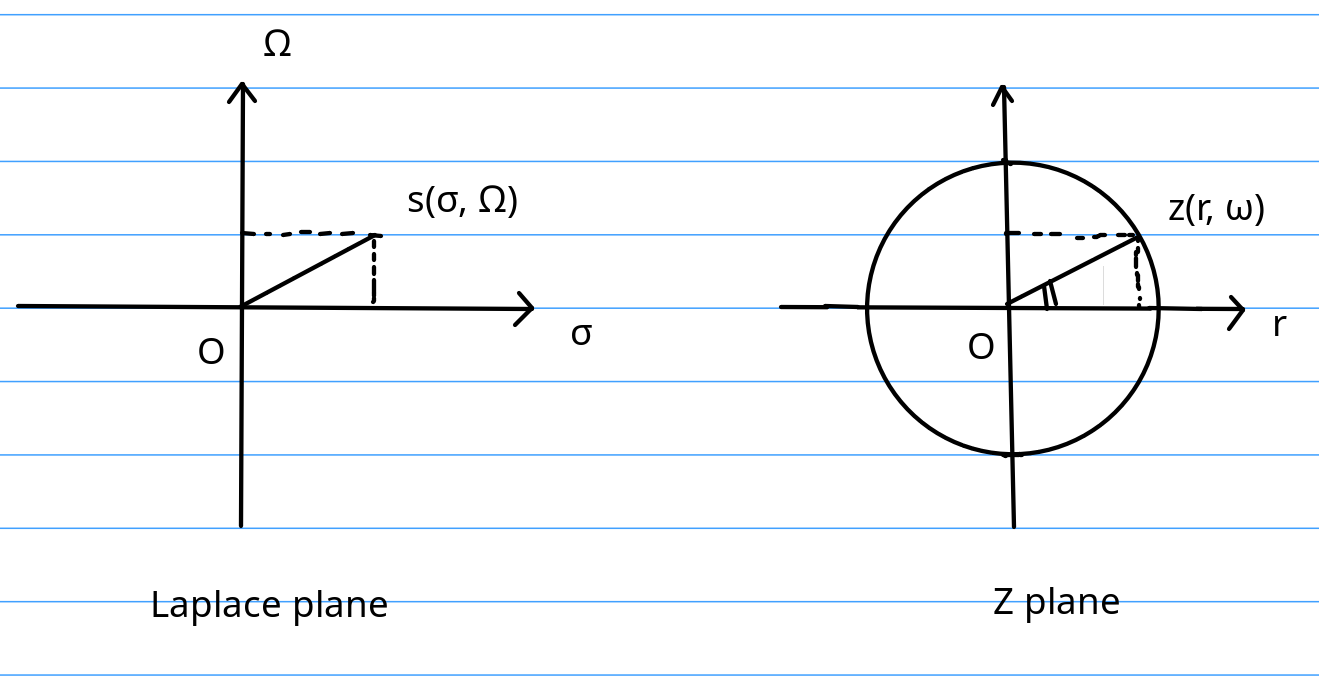
\includegraphics[width=13cm]{splane.png}
    \end{center}
    \end{figure}
\\Ta có thể nhận thấy rằng phép biến đổi trên có dạng giống với phép biến đổi giữa hai hệ tọa độ Cartesian và hệ tọa độ cực (Polar Coordinate). Ta thử áp dụng phép đổi biến giữa hai hệ tọa độ này để tìm mối liên hệ giữa các biến tương ứng như sau:
\begin{equation*}
    \begin{cases}
        r=\sqrt{\sigma^{2}+\Omega^{2}} \\
        \omega = \arctan{\left(\frac{\Omega}{\sigma}\right)}
    \end{cases}
\end{equation*}
Khi $\Omega\to0$ thì $\arctan\left(\frac{\Omega}{\sigma}\right)\approx\frac{\Omega}{\sigma}$, khi đó ta thu được phương trình tuyến tính liên hệ giữa $\omega$ và $\Omega$:
$$\omega=\frac{\Omega}{\sigma}$$
Ta quay trở lại phương trình liên hệ giữa $\Omega$ và $\omega$ đã chứng minh ở câu $1$, với điều kiện cả hai tần số $\Omega$ và $\omega$ đều xấp xỉ $0$, ta có:
\begin{equation*}
    \begin{split}
        \Omega=C\frac{2r\sin{\omega}}{r^{2}+2r\cos{\omega}+1}\approx C\frac{2r\omega}{r^2+2r+1} \Rightarrow C=\frac{\Omega(r+1)^2}{2r\omega}=\frac{\sigma(r+1)^2}{2r}
    \end{split}
\end{equation*}
Vậy với điều kiện $\Omega\to0$ và $\omega\to0$ thì: $$C=\frac{\sigma(r+1)^2}{2r}$$ sẽ cho ra kết quả $\Omega$ và $\omega$ phụ thuộc tuyến tính với nhau.
\end{document}